\graphicspath{{figs/3b}}

\chapter{Approximate Inference in Classification}

This chapter extends the exploration of Bayesian Deep Learning. Building upon the previous chapter, it delves into the complexities of classification tasks. The focus here is on the challenges associated with these tasks, particularly the lack of a closed-form solution for the posterior distribution in Logistic Regression. The chapter conducts a comparative analysis of different approximate inference techniques, including Laplacian approximation and variational inference, applied to binary classification problems. This exploration is crucial for gaining insights into the application of Bayesian methods in more complex machine learning scenarios, representing a substantial advancement from the linear regression models discussed earlier.

\section{Bayesian Logistic Regression}

In this section, our initial focus is on Bayesian Logistic Regression. We begin by highlighting he difference between the continuous predictions found in linear regression models and the discrete class label predictions characteristic of classification models. Specifically, we introduce binary classification through logistic regression and explore several methods for approximating the posterior distribution, as the posterior distribution is no longer tractable due to the absence of conjugacy between the likelihood and the prior. 

\subsection{Maximum-A-Posteriori Estimate}
\paragraph{1.1. Analyze the results provided by \Cref{fig:logreg_map}. Looking at $p(y=1 | x, \mathbf{w}_{\textrm{MAP}})$, what can you say about points far from train distribution?}

Approximating $p(\mathbf{w} | \mathbf{X}, \mathbf{Y})$ with a Dirac delta function is essentially akin to approximating the predictive distribution using $\mathbf{w}_{\textrm{MAP}}$, meaning $p(y=1 | x, \mathbf{w}_{\textrm{MAP}}) \approx p(y=1 | x, \mathbf{Y})$. This approximation is quite straightforward. 

\begin{figure}[H]
    \centering
    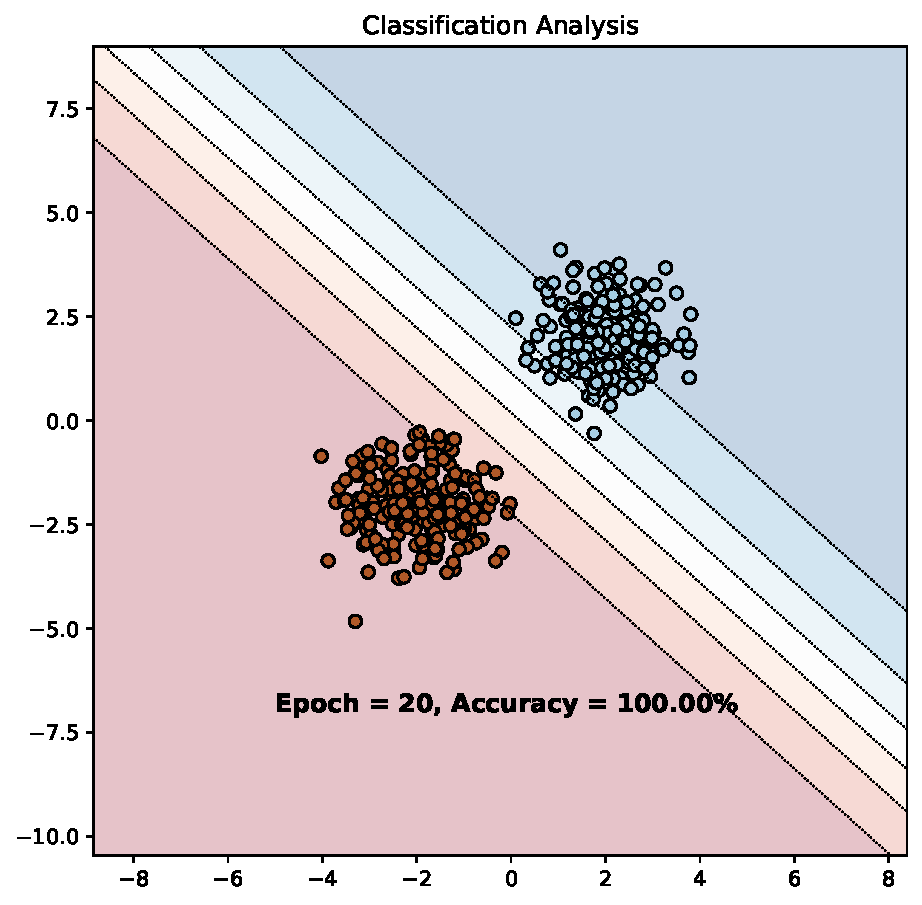
\includegraphics[width=0.45\textwidth]{logreg_map.pdf}
    \caption{Illustration of a Bayesian Logistic Regression model applied to a binary classification task with uncertainty display, with a weight decay of $5 \times 10^{-2}$. Two distinct data point clusters — blue and red — represent separate classes, while the surrounding shaded areas reflect the model's predictive uncertainty, with lighter shades indicating lower confidence.}
    \label{fig:logreg_map}
\end{figure}

As depicted in \Cref{fig:logreg_map}, the boundary decision remains linear and the model's uncertainty doesn't significantly increase far from the training data. Essentially, it provides a confidence measure for the linear boundary. This indicates that the point-wise estimate of the parameters can only confidently assign points to their respective classes but lacks the capacity to provide nuanced uncertainty measures for points that deviate far from the training data distribution. Thus, this approach is not effective in assessing the uncertainty of outliers or points not well-represented in the training set.

\subsection{Laplace Approximation}
\paragraph{1.2. Analyze the results provided by \Cref{fig:laplace_approx}. Compared to previous MAP estimate, how does the predictive distribution behave?}

Compared to the MAP estimate, Bayesian Logistic Regression using the Laplace approximation better captures uncertainty about the model parameters. While the MAP estimate gives a single point estimate of the weights ($\mathbf{w}_{\textrm{MAP}}$) and therefore a single decision boundary, the Laplace approximation treats the weights as a normal distribution. This distribution is centered around $\mathbf{w}_{\textrm{MAP}}$ and has a covariance matrix based on the Hessian of the log posterior. This approach allows for uncertainty in the decision boundary, as clearly shown in \Cref{fig:laplace_approx}.

For instance, moving in the southwest direction away from the red cluster — directly opposite the blue cluster — the model exhibits high confidence that this region predominantly consists of red points. The same holds true for the blue cluster. This directional certainty reflects the model's aleatoric uncertainty, which is the irreducible uncertainty inherent in the observations due to noise or other stochastic effects. Conversely, if we move sideways, out of the line between the clusters to areas with less or no data, the model becomes less certain. This reflects the epistemic uncertainty of our model, relating to what the model doesn't know about its own parameters.

\begin{figure}[H]
    \centering
    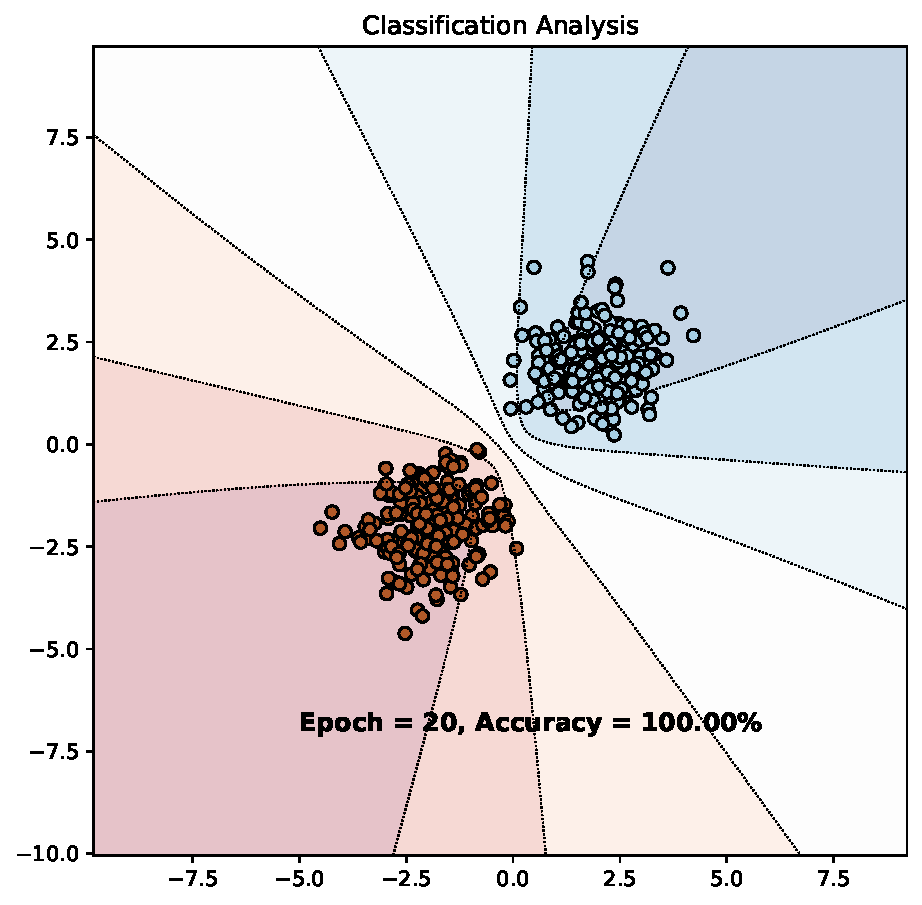
\includegraphics[width=0.45\textwidth]{laplace_approx.pdf}
    \caption{Illustration of a Bayesian Logistic Regression with Laplace approximation model applied to a binary classification task, with a weight decay of $5 \times 10^{-2}$.}
    \label{fig:laplace_approx}
\end{figure}


\paragraph{1.3. Comment the effect of the regularisation hyper-parameter \texttt{WEIGHT\_DECAY}.}

The weight decay hyper-parameter controls the complexity of the model. It adds a penalty to the loss function for large weights, effectively encouraging the model to maintain smaller weight values, which usually help prevent overfitting. In Bayesian terms, weight decay corresponds to the precision (inverse variance) of the prior distribution over the weights. A higher weight decay value means a tighter prior, which pulls the weights closer to zero, unless the data provides strong evidence to the contrary. This can affect the predictive distribution by potentially making it more conservative. As a result, the decision boundary may be less flexible and the model may exhibit higher uncertainty, especially in regions far from the training data. This behavior is verified in \Cref{fig:weight_decay}. When the weight decay is too high, it results in increased predictive uncertainty (wider shaded areas), whereas when it's too low, it results in high confidence (narrower shaded areas), which may not be justified for unseen data.

\begin{figure}[H]
    \centering
    \begin{subfigure}{0.45\textwidth}
        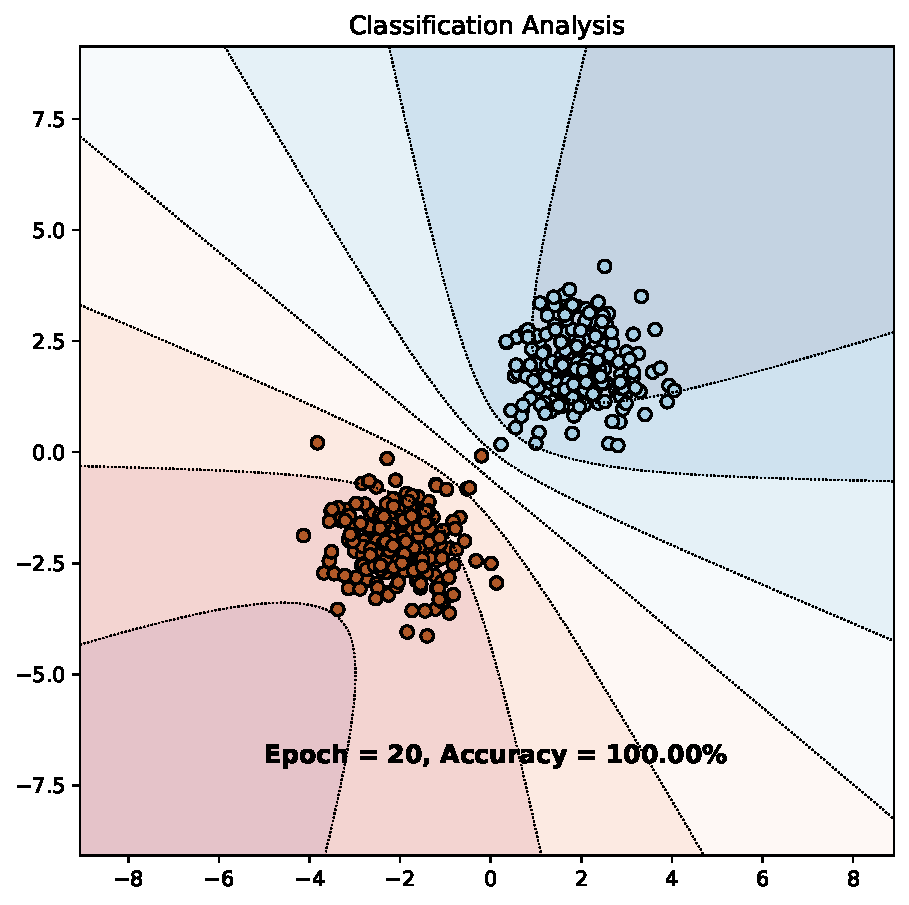
\includegraphics[width=\textwidth]{laplace_approx_0.5.pdf}
        \caption{}
        \label{subfig:weight_decay_high}
    \end{subfigure}%
    \begin{subfigure}{0.45\textwidth}
        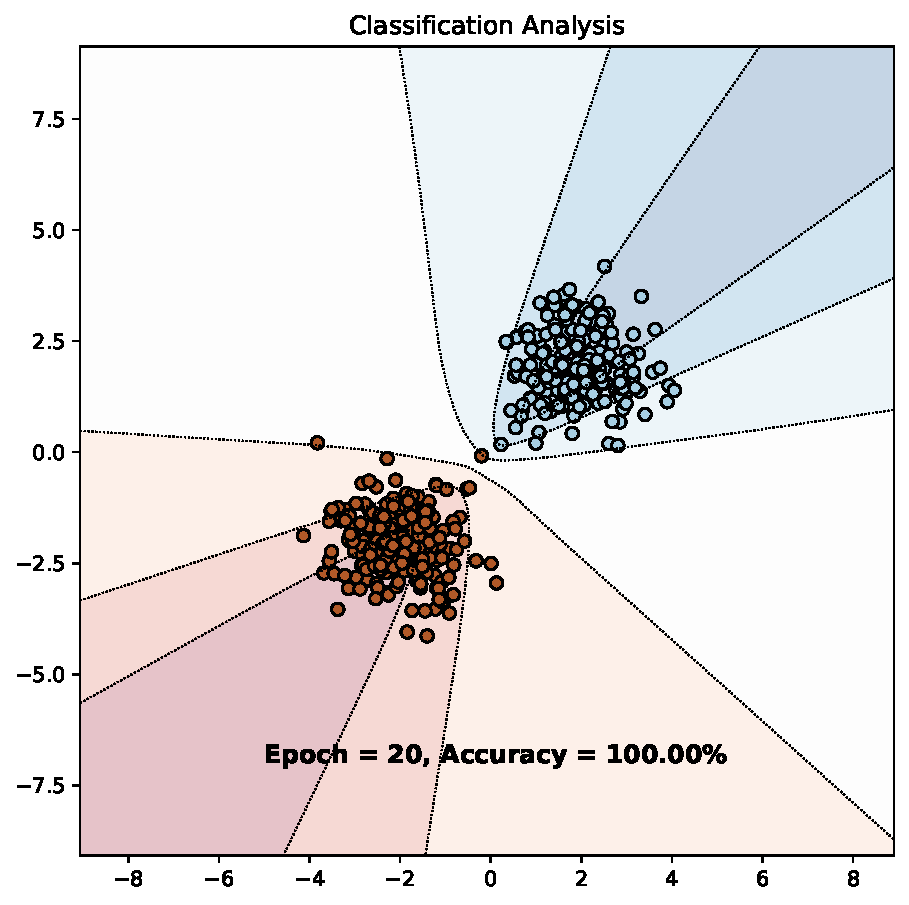
\includegraphics[width=\textwidth]{laplace_approx_5e-05.pdf}
        \caption{}
        \label{subfig:weight_decay_low}
    \end{subfigure}%
    \caption{Illustration of a Bayesian Logistic Regression with Laplace approximation model applied to a binary classification task, with a weight decay of (a) $0.5$ and (b) $5 \times 10^{-5}$.}
    \label{fig:weight_decay}
\end{figure}

\subsection{Variational Inference}
\paragraph{1.4. Comment the code of the \texttt{VariationalLogisticRegression} and \texttt{LinearVariational} classes.}

\noindent\texttt{LinearVariational} represents a single linear layer with variational inference applied. It approximates the weights and biases of the layer with distributions rather than fixed values.
\begin{itemize}
    \item The class is initialized with the variational parameters for the weights (\texttt{w\_mu}, \texttt{w\_rho}) and biases (\texttt{b\_mu}) of the layer, i.e. the parameters we want to learn. \texttt{prio\_var} represents the variance of the prior distribution ($\sigma^2_p$), which specify our prior belief about the distribution of the weights. 
    \item The \texttt{sampling} method uses the reparametrization trick to sample from the variational posterior distribution for the weights $\boldsymbol{w}_{i} \sim \mathcal{N}(\mu_{i}, \sigma_{i}^2)$. To do so, we sample from a centered isotropic multivariate Gaussian where $ \sigma^2 = \log(1 + e^{\rho}) $ to avoid numerical issues. Thus, $ \boldsymbol{w}_{i} = \mu_{i}+ \sigma_{i} \odot \boldsymbol{\varepsilon}_s $, where $\boldsymbol{\varepsilon}_s \sim \mathcal{N}(0, 1)$ is a Gaussian noise. The reparametrization trick allows the gradient of the loss function to backpropagate through the randomness of the sampling process. 
    \item The \texttt{kl\_divergence} method calculates the Kullback-Leibler divergence between the variational posterior and the prior distribution for the weights: \[
    \textrm{KL}\left[q_{\theta}(\boldsymbol{w}) \Vert p(\boldsymbol{w}) \right]= \log\left(\frac{\sigma_{p}}{\sigma_{i}}\right) + \frac{\sigma_i^2+\mu_i^2}{2\sigma_{p}^2} - \frac{1}{2} \]
    where $\sigma^2_p$ is the variance of our prior distribution $p(\boldsymbol{w})$ and $(\mu_i, \sigma^2_i)$ the mean and variance of the variational distribution $q_{\theta}(\boldsymbol{w})$.
    \item The \texttt{forward} method defines the forward pass by performing a linear transformation, i.e. $w^T x + b$. We sample the weights then compute the output of the layer using the sampled weights and the mean of the biases.
\end{itemize}

\noindent\texttt{VariationalLogisticRegression} represents a logistic regression model using variational inference:
\begin{itemize}
    \item The class is initialized with one linear variational layer used to perform the linear transformation in logistic regression.
    \item The \texttt{forward} method defines the forward pass for the logistic regression model by returning $f(x) = \sigma(w^T x + b)$ where $\sigma$ is the sigmoid function. 
    \item The \texttt{kl\_divergence} method simply calls the same method of the \texttt{LinearVariational} layer to obtain the KL divergence term for the loss computation.
\end{itemize}

\paragraph{1.5. Comment the code of the training loop, especially the loss computation. Analyze the results provided by \Cref{fig:logreg_variational}. Compared to previous MAP estimate, how does the predictive distribution behave? What is the main difference between the Variational approximation and the Laplace approximation?}

The training loop uses a standard PyTorch format. The loss function calculates the Evidence Lower Bound (ELBO), which we want to maximize. In theory, we aim to maximize the likelihood of the data directly, but this is often intractable due to the integral over the weights. Therefore, we compute the Kullback-Leibler divergence $\textrm{KL}(q_{\boldsymbol{\theta}}(\boldsymbol{w}) \Vert p(\boldsymbol{w}))$ between the variational distribution $q_{\theta}(\boldsymbol{w})$ and the prior distribution $p(\boldsymbol{w})$. This acts as a regularization term, encouraging the variational distribution to be similar to the prior distribution. It represents the information lost when using $q_{\theta}(\boldsymbol{w})$ to approximate $p(\boldsymbol{w})$, which we want to minimize. 

To ensure the model fits the data effectively, we compute the negative log-likelihood $NLL(\boldsymbol{\theta}; \mathcal{D})$ of the data under the model parameterized by the weights sampled from $q_{\theta}(w)$. This is done using a binary cross-entropy loss. Subsequently, as maximizing ELBO is equivalent to minimizing: \[ \mathcal{L}_{\textrm{VI}}(\boldsymbol{\theta}; \mathcal{D}) = NLL(\boldsymbol{\theta}; \mathcal{D}) + \textrm{KL}(q_{\boldsymbol{\theta}}(\boldsymbol{w})\vert\vert p(\boldsymbol{w})),\] we employ gradient descent to update the parameters of the variational distribution to better approximate the true posterior.

The results of this variational approximation yield decision boundaries that are less rounded, falling between Maximum a Posteriori and Laplace approximation, as visualized in \Cref{fig:logreg_variational}. It provides a better encompassing of noisy data points, and all training points fall within regions of high confidence. Consequently, it yields a decision frontier that is noticeably distinct in the central area while effectively accounting for aleatoric uncertainty.

\begin{figure}[H]
    \centering
    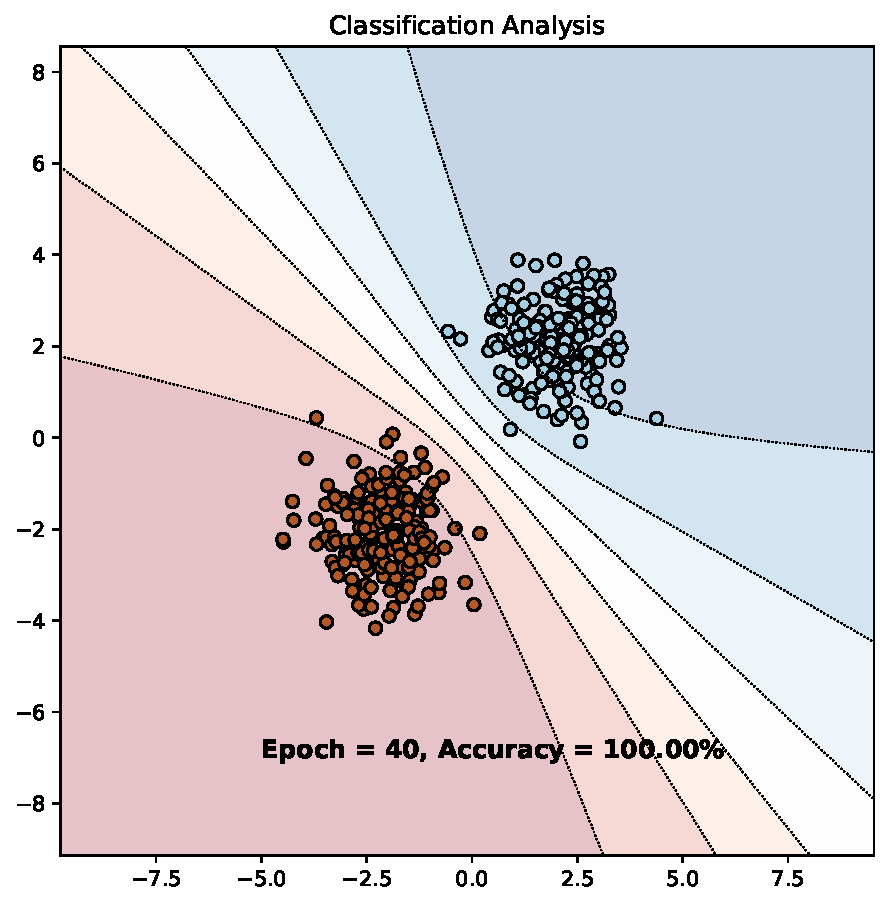
\includegraphics[width=0.45\textwidth]{logreg_variational.pdf}
    \caption{Illustration of a Variational Logistic Regression model applied to a binary classification task.}
    \label{fig:logreg_variational}
\end{figure}

Compared to a Maximum a Poseteriori estimate, the variational approach does not just find the most probable weights (as MAP does) but instead approximates the entire posterior distribution over the weights. In the variational approach, the predictive distribution captures the model's uncertainty about its predictions.

Compared to the Laplace approximation, the variational approximation actively optimizes a parameterized distribution to closely resemble the true posterior, with resemblance quantified by the KL divergence. This optimization typically involves a more complex objective function. On the other hand, Laplace approximation passively fits a Gaussian distribution around the MAP estimate, relying on the curvature of the log-posterior at that point. It assumes that the posterior is locally Gaussian and primarily focuses on finding the MAP estimate and computing the Hessian at that location.

\section{Bayesian Neural Networks}

In this section, we illustrate the extension of Bayesian methods to neural network architecture, with a specific focus on applying variational inference to a Multi-Layer Perceptron. Here, we practically apply the concepts introduced in the previous section to showcase their effectiveness in dealing with complex, non-linear datasets.

\subsection{Variational Inference with Bayesian Neural Networks}
\paragraph{2.1. Analyze the results showed on \Cref{fig:mlp_variational}.}

By applying Bayesian principles to a neural network with two hidden layers, we create a model capable of capturing intricate patterns within the data. In this context, each neuron's weight is treated as a random variable, representing our uncertainty about its true value. Consequently, we obtain a complex and non-linear decision boundary. Notably, the shaded regions, indicating the model's predictive uncertainty, reveal that the model demonstrates high confidence near the training data points and experiences increased uncertainty as it moves further away. Interestingly, this behavior leads to the emergence of ''clusters'' resembling the moon-shaped patterns found in the dataset. Moreover, this approach offers explainability, as it provides outputs that are not just binary but instead resemble the level of confidence one might have when predicting the locations of new data points.

\begin{figure}[H]
    \centering
    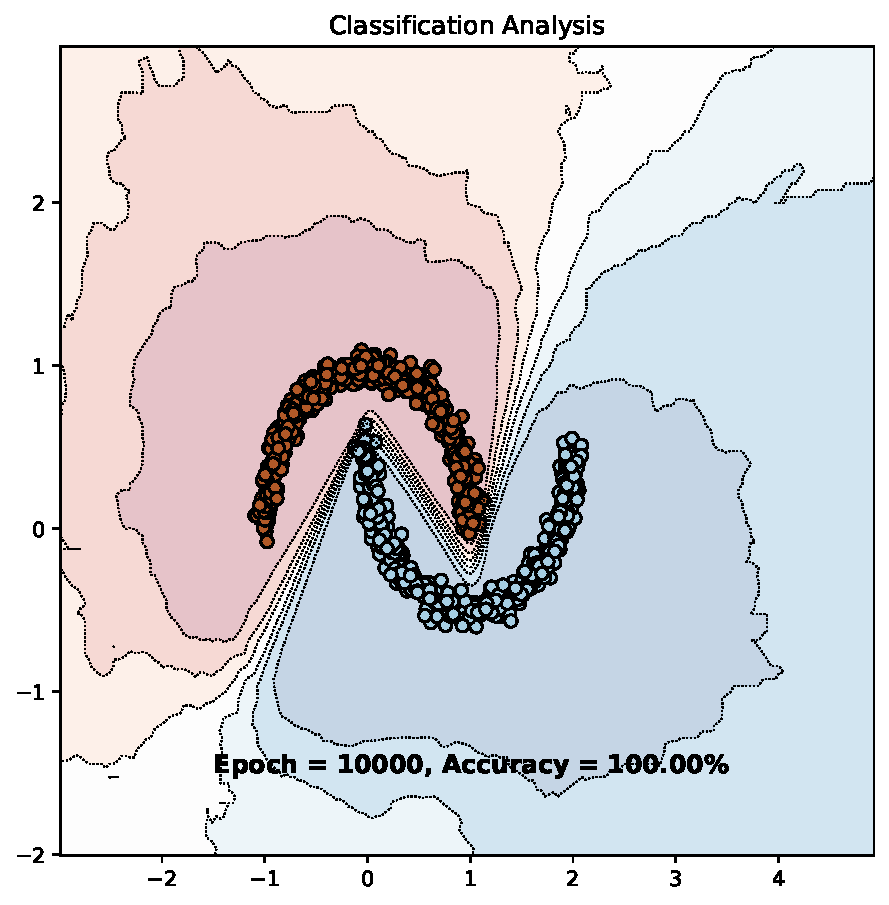
\includegraphics[width=0.45\textwidth]{mlp_variational.pdf}
    \caption{Illustration of a Bayesian Neural Network model applied to a binary classification task.}
    \label{fig:mlp_variational}
\end{figure}

\subsection{Monte Carlo Dropout}
\paragraph{2.2. Again, analyze the results showed on \Cref{fig:dropout}. What is the benefit of MC Dropout variational inference over Bayesian Logistic Regression with variational inference?}

Monte Carlo dropout is a technique that aligns with variational inference in Bayesian neural networks, where the dropout mechanism acts as a variational distribution for the network weights. Essentially, dropout introduces Bernoulli random variables, leading to a posterior predictive distribution that accounts for weight uncertainty. The formula for the predictive distribution of an output $ y $ for a new input $ x^* $ is: \[ p(y | x^*, \mathbf{X}, \mathbf{Y}) \approx \frac{1}{S} \sum_{s \in S} p(y^* | x^*, \mathbf{w}_s), \] where $ \mathbf{w}_s $ represents the network weights after dropout, and $ S $ is the number of MC samples or dropout iterations.

The results, shown in \Cref{subfig:mcdropout}, include a decision boundary with adjacent bands indicating the model's confidence levels. These bands are formed by applying dropout during inference and averaging results from multiple stochastic passes. This approach illustrates the model's uncertainty in predictions, which contrast to the smooth gradients of deterministic neural networks (shown in \Cref{subfig:dropout}). The speckled appearance of uncertainty regions in the plot reflects how confidence varies across different input regions, due to the randomness introduced by MC Dropout. Incorporating MC Dropout in a standard neural network effectively turns it into Bayesian-like model, capable of expressing uncertainty in predictions. This approach not only allows the network to learn complex decision boundaries but also provides estimates of uncertainty, something often missing in regular neural networks. This probabilistic interpretation can lead to more informed decisions, as it shows how reliable the network's predictions are across different input areas.

\begin{figure}[H]
    \centering
    \begin{subfigure}{0.45\textwidth}
        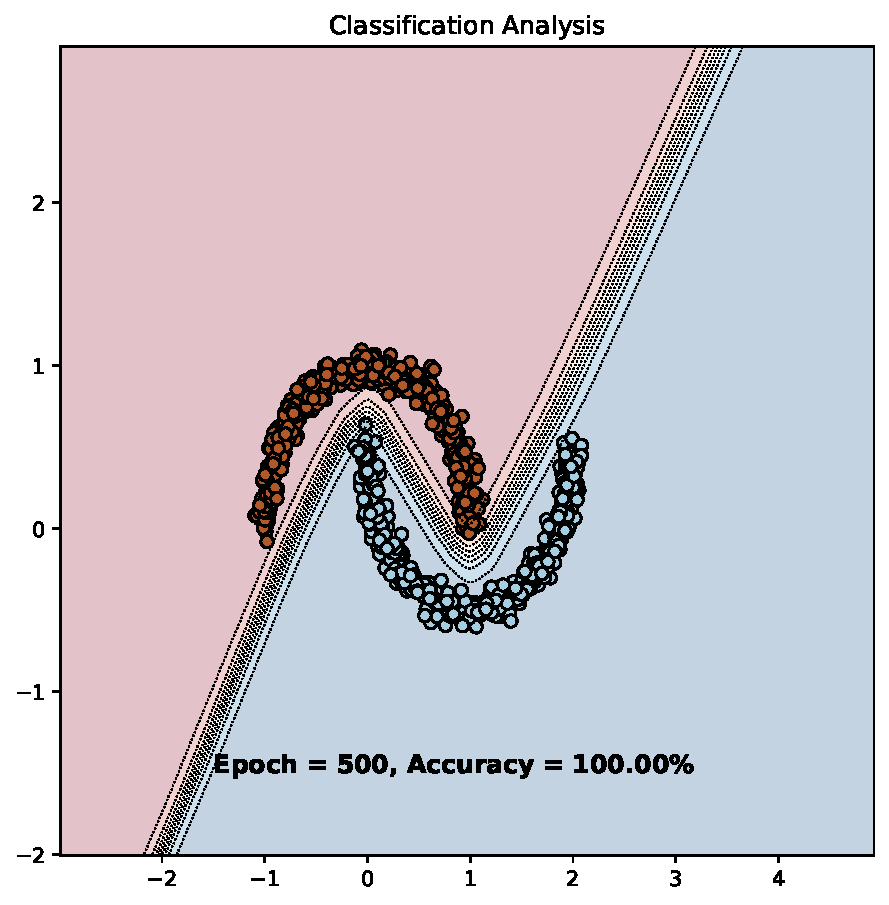
\includegraphics[width=\textwidth]{dropout.pdf}
        \caption{}
        \label{subfig:dropout}
    \end{subfigure}%
    \begin{subfigure}{0.45\textwidth}
        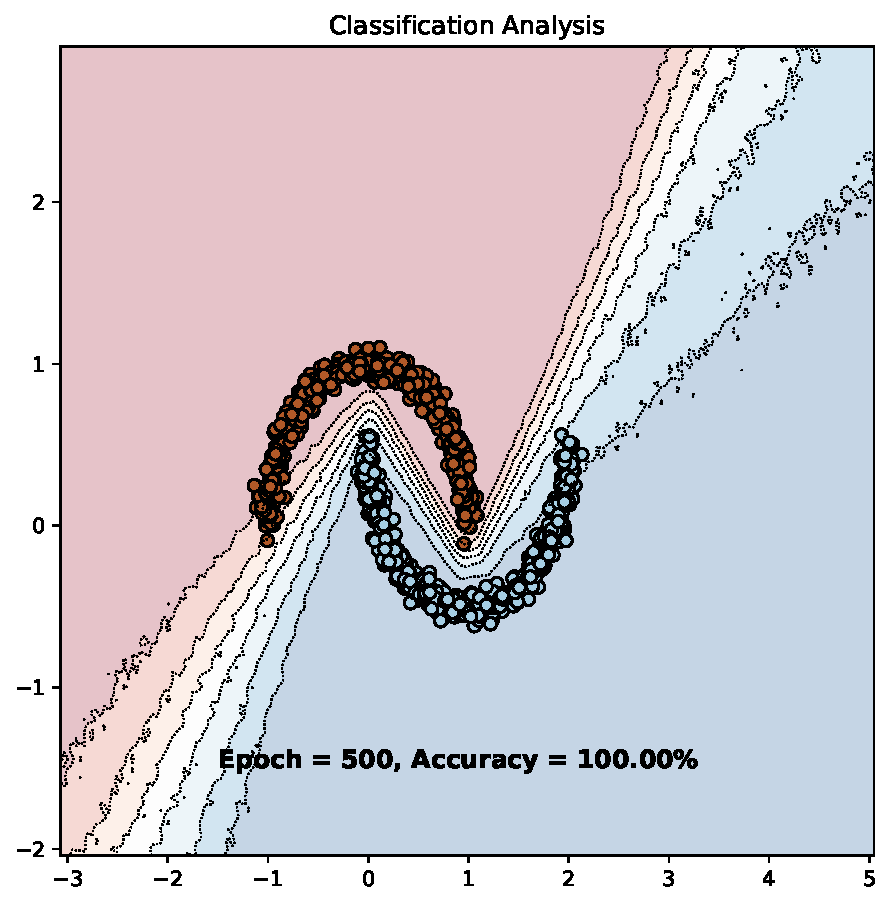
\includegraphics[width=\textwidth]{mcdropout.pdf}
        \caption{}
        \label{subfig:mcdropout}
    \end{subfigure}%
    \caption{Illustration of a Bayesian Neural Network model applied to a binary classification task using (a) dropout and (b) Monte-Carlo dropout.}
    \label{fig:dropout}
\end{figure}
